\documentclass[a4paper,11pt]{article}
\usepackage[utf8]{inputenc}
\usepackage[T1]{fontenc}
\usepackage{amsmath,amssymb}
\usepackage[a4paper,left=2cm,right=2cm,top=3.6cm,bottom=2.3cm,headheight=1.1cm,headsep=0.6cm,footskip=1cm]{geometry}
\usepackage{xcolor}
\usepackage{tikz}
\usetikzlibrary{calc,arrows.meta,positioning,shapes.geometric,matrix}
\usepackage{fancyhdr}
\usepackage{lastpage}
\usepackage{tabularx}
\usepackage{array}
\usepackage[most]{tcolorbox}
\usepackage{enumitem}
\usepackage{needspace}

% ---------- palet sky (Sky-800 dan Sky-200) ----------
\definecolor{mainc}{HTML}{075985}
\definecolor{accc}{HTML}{0284C7}
\definecolor{skyl}{HTML}{BAE6FD}
\definecolor{deepc}{HTML}{082F49}
\definecolor{softbg}{HTML}{F0F9FF}
\definecolor{warmc}{HTML}{D97706}
\definecolor{brick}{HTML}{B91C1C}
\newcommand{\dis}{\displaystyle}

\setlength{\parindent}{0pt}
\renewcommand{\arraystretch}{1.35}

\tikzset{
  ar/.style={-{Stealth[length=1.8mm]},thick,mainc},
  box/.style={draw=mainc,thick,rounded corners=3pt,fill=softbg,align=center,inner sep=4pt}
}

% ---------- header ----------
\pagestyle{fancy}
\fancyhf{}
\renewcommand{\headrulewidth}{0pt}
\fancyhead[L]{%
  \begin{tikzpicture}[remember picture,overlay]
    \fill[mainc] ([yshift=-1.2cm]current page.north west) rectangle ([yshift=-3.15cm]current page.north east);
    \fill[skyl] ([yshift=-3.15cm]current page.north west) rectangle ([yshift=-3.3cm]current page.north east);
  \end{tikzpicture}%
  \color{white}\bfseries\large Latihan Soal Limit Fungsi}
\fancyhead[R]{\color{white}\small Diunduh dari website \textbf{Math1729}\ \,|\,\ 5 Oktober 2026}
\fancyfoot[L]{\small\color{mainc}Math1729 --- Limit Fungsi}
\fancyfoot[R]{\small\color{mainc}Halaman \thepage\ dari \pageref{LastPage}}

% ---------- komponen ----------
\newcounter{no}
\newcommand{\bagian}[2]{\par\Needspace{6\baselineskip}\vspace{1.0em}\noindent
  \begin{tcolorbox}[colback=mainc,colframe=mainc,coltext=white,boxrule=0pt,arc=2pt,left=6pt,right=6pt,top=3pt,bottom=3pt]
  \textbf{#1}\hfill{\small #2}\end{tcolorbox}\setcounter{no}{0}\par\vspace{-0.3em}}
\newcommand{\tingkat}[2]{\par\Needspace{7\baselineskip}\vspace{0.6em}\noindent
  {\color{accc}\rule{3pt}{1.1em}}\ {\color{mainc}\bfseries #1}\ {\small\color{gray}--- #2}\par\vspace{0.1em}}
\newcommand{\soal}[2]{\par\vspace{0.75em}\stepcounter{no}\noindent
  \begin{minipage}[t]{1.8em}\textbf{\theno.}\end{minipage}%
  \begin{minipage}[t]{\dimexpr\linewidth-1.8em\relax}#1\par\vspace{0.35em}#2\end{minipage}\par}
\newcommand{\poin}[1]{\hfill{\small\color{mainc}[#1 poin]}}
\newcommand{\gbr}[2]{\noindent\begin{minipage}[t]{0.56\linewidth}#1\end{minipage}\hfill\raisebox{\ht\strutbox}{\begin{minipage}[t]{0.41\linewidth}\vspace{0pt}\centering#2\end{minipage}}}
\newcommand{\pil}[5]{\begin{tabularx}{\linewidth}{@{}*{5}{X}@{}}\textbf{A.}\;#1 & \textbf{B.}\;#2 & \textbf{C.}\;#3 & \textbf{D.}\;#4 & \textbf{E.}\;#5\end{tabularx}}
\newcommand{\pilx}[5]{\begin{tabularx}{\linewidth}{@{}*{3}{X}@{}}\textbf{A.}\;#1 & \textbf{B.}\;#2 & \textbf{C.}\;#3\\[10pt] \textbf{D.}\;#4 & \textbf{E.}\;#5 & \end{tabularx}}
\newcommand{\jwb}{\hfill Jawaban: \rule{4.5cm}{0.4pt}}

\begin{document}
\thispagestyle{fancy}

\begin{center}
  {\color{mainc}\fontsize{22}{26}\selectfont\bfseries Latihan Soal Limit Fungsi\par}
  \vspace{2pt}
  {\color{accc}\large Limit Aljabar dan Trigonometri, Limit Tak Hingga, Bilangan $e$, Kekontinuan, Teorema Apit, dan Penalaran Limit\par}
\end{center}
\vspace{2pt}
\begin{tcolorbox}[colback=softbg,colframe=mainc!40,boxrule=0.6pt,arc=3pt,left=8pt,right=8pt,top=5pt,bottom=5pt]
\noindent\textbf{Nama} : \rule{4.6cm}{0.4pt}\hfill\textbf{Kelas} : \rule{2.2cm}{0.4pt}\hfill\textbf{Skor} : \rule{2.2cm}{0.4pt}
\end{tcolorbox}
\vspace{2pt}
\begin{tcolorbox}[colback=white,colframe=accc,boxrule=0.8pt,arc=3pt,left=8pt,right=8pt,top=4pt,bottom=4pt,title={\bfseries Petunjuk Pengerjaan},coltitle=white,fonttitle=\small]
\small
\begin{enumerate}[leftmargin=1.4em,itemsep=1pt,topsep=1pt]
\item Soal terdiri atas \textbf{20 pilihan ganda} (5 mudah, 6 sedang, 7 sulit, 2 HOTS), \textbf{5 isian singkat} (2 sedang, 3 sulit), dan \textbf{5 uraian (essay)} (2 sedang, 2 sulit, 1 HOTS). Soal disusun berjenjang dan memakai bentuk yang sejalan dengan UTBK-SNBT 2026: pilihan ganda lima opsi, pilihan majemuk kompleks (benar/salah), kecukupan data, soal berkonteks dengan gambar atau grafik, dan isian singkat. Alokasi waktu yang disarankan: 120 menit.
\item Skor: pilihan ganda 2 poin, isian singkat 4 poin, uraian 8 poin per soal (total 100 poin). Tidak ada pengurangan skor untuk jawaban salah.
\item Notasi: sudut pada fungsi trigonometri dinyatakan dalam radian; $\lfloor x\rfloor$ adalah bilangan bulat terbesar yang tidak melebihi $x$; $x\to a^-$ dan $x\to a^+$ berturut-turut berarti mendekati dari kiri dan dari kanan. Pada grafik, titik berlubang berarti titik itu tidak dimiliki grafik, sedangkan titik penuh adalah nilai fungsi di titik tersebut. Gambar tidak selalu digambar sesuai skala.
\item Bilangan ribuan ditulis dengan tanda titik dan bilangan desimal dengan tanda koma. Pada isian singkat, tuliskan hanya jawaban akhir (pecahan paling sederhana, bentuk akar, atau bentuk eksponen bila perlu).
\item Kalkulator tidak diperkenankan. Aturan L'H\^opital boleh dipakai kecuali soal menyatakan lain.
\end{enumerate}
\end{tcolorbox}

% =====================================================================
\bagian{A. Pilihan Ganda}{20 soal $\times$ 2 poin = 40 poin. Pilih satu jawaban yang paling tepat.}

\tingkat{Tingkat Mudah}{soal 1 sampai 5}
\soal{\gbr{Perhatikan grafik fungsi $f$ pada gambar. Pernyataan berikut yang \textbf{benar} adalah \dots.}{%
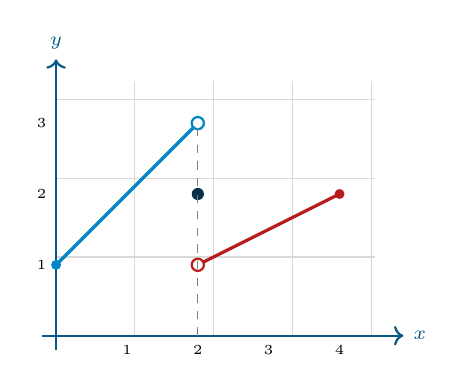
\begin{tikzpicture}[x=0.9cm,y=0.9cm]
\draw[gray!30] (0,0) grid (4.5,3.6);
\draw[->,thick,mainc] (-0.2,0)--(4.9,0) node[right,font=\scriptsize]{$x$};
\draw[->,thick,mainc] (0,-0.2)--(0,3.9) node[above,font=\scriptsize]{$y$};
\draw[accc,very thick] (0,1)--(2,3);
\draw[brick,very thick] (2,1)--(4,2);
\fill[accc] (0,1) circle (1.8pt);
\fill[brick] (4,2) circle (1.8pt);
\draw[fill=white,draw=accc,thick] (2,3) circle (2.2pt);
\draw[fill=white,draw=brick,thick] (2,1) circle (2.2pt);
\fill[deepc] (2,2) circle (2.2pt);
\draw[dashed,gray] (2,0)--(2,3);
\foreach \i in {1,2,3}{\node[font=\tiny,left] at (0,\i){$\i$};}
\foreach \i in {1,2,3,4}{\node[font=\tiny,below] at (\i,0){$\i$};}
\end{tikzpicture}}}{\begin{tabularx}{\linewidth}{@{}lX@{}}
\textbf{A.} & $\dis\lim_{x\to2}f(x)=2$\\
\textbf{B.} & $\dis\lim_{x\to2}f(x)=3$\\
\textbf{C.} & $\dis\lim_{x\to2^+}f(x)=f(2)$\\
\textbf{D.} & $\dis\lim_{x\to2^-}f(x)-\lim_{x\to2^+}f(x)=2$\\
\textbf{E.} & $f$ kontinu di $x=2$
\end{tabularx}}
\soal{Diketahui $\dis\lim_{x\to3}f(x)=4$ dan $\dis\lim_{x\to3}g(x)=-2$. Nilai $\dis\lim_{x\to3}\dfrac{f(x)\,g(x)+6}{f(x)-g(x)}$ adalah \dots.}{\pil{$-3$}{$-1$}{$-\frac13$}{$\frac13$}{$3$}}
\soal{Nilai $\dis\lim_{x\to-2}\dfrac{x^2+5x+6}{x^2-x-6}$ adalah \dots.}{\pil{$-1$}{$-\frac15$}{$0$}{$\frac15$}{$1$}}
\soal{Nilai $\dis\lim_{x\to\infty}\dfrac{(2x-1)(x+3)}{(x-2)(3x+1)}$ adalah \dots.}{\pil{$0$}{$\frac13$}{$\frac32$}{$2$}{$\frac23$}}
\soal{Tentukan nilai kebenaran tiga pernyataan berikut (B = benar, S = salah), berurutan dari (i) sampai (iii).\par\smallskip
(i) $\dis\lim_{x\to0}\dfrac{\tan4x}{\sin2x}=2$.\par
(ii) $\dis\lim_{x\to\infty}\dfrac{\sin x}{x}=1$.\par
(iii) $\dis\lim_{x\to\infty}\dfrac{2x^2+1}{x^2-3}=2$.}{\pilx{B, S, B}{B, B, S}{S, S, B}{S, B, B}{B, B, B}}

\tingkat{Tingkat Sedang}{soal 6 sampai 11}
\soal{Nilai $\dis\lim_{x\to1}\dfrac{\sqrt{x+3}-2}{\sqrt{x+8}-3}$ adalah \dots.}{\pil{$\frac23$}{$\frac32$}{$2$}{$3$}{$6$}}
\soal{Nilai $\dis\lim_{x\to0}\dfrac{\cos2x-\cos6x}{x^2}$ adalah \dots.}{\pil{$8$}{$12$}{$16$}{$20$}{$32$}}
\soal{Nilai $\dis\lim_{x\to\infty}\left(\dfrac{x+3}{x-1}\right)^{2x}$ adalah \dots.}{\pil{$e$}{$e^2$}{$e^4$}{$e^6$}{$e^8$}}
\soal{\gbr{Dua menara pemantau berada di $A(-4,2)$ dan $B(2,3)$ (satuan km). Sebuah jalan lurus berimpit dengan sumbu-$x$. Seorang pelari berlari menjauh sepanjang jalan itu dan posisinya $P(x,0)$ dengan $x>0$. Untuk $x$ yang sangat besar, selisih jarak $PA-PB$ mendekati \dots\ km.}{%
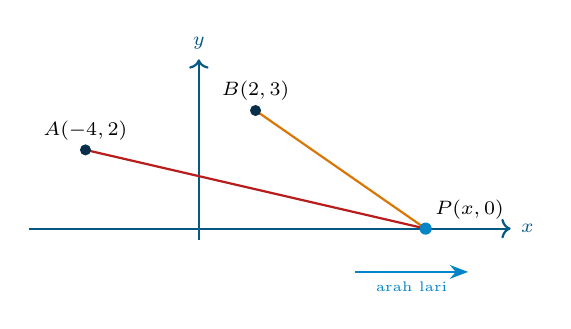
\begin{tikzpicture}[x=0.36cm,y=0.5cm]
\draw[->,thick,mainc] (-6,0)--(11,0) node[right,font=\scriptsize]{$x$};
\draw[->,thick,mainc] (0,-0.3)--(0,4.3) node[above,font=\scriptsize]{$y$};
\coordinate (A) at (-4,2); \coordinate (B) at (2,3); \coordinate (P) at (8,0);
\draw[brick,thick] (A)--(P);
\draw[warmc,thick] (B)--(P);
\fill[deepc] (A) circle (2pt) (B) circle (2pt);
\fill[accc] (P) circle (2.2pt);
\node[font=\scriptsize,above] at (A) {$A(-4,2)$};
\node[font=\scriptsize,above] at (B) {$B(2,3)$};
\node[font=\scriptsize,above right] at (P) {$P(x,0)$};
\draw[-{Stealth},thick,accc] (5.5,-1.1)--(9.5,-1.1) node[midway,below,font=\tiny]{arah lari};
\end{tikzpicture}}}{\pil{$1$}{$2$}{$5$}{$6$}{$7$}}
\soal{\gbr{Fungsi $f$ memenuhi $4x-5\le f(x)\le x^2-1$ untuk semua bilangan real $x$ (grafik $f$ terletak di antara dua kurva pada gambar). Nilai $\dis\lim_{x\to2}f(x)$ adalah \dots.}{%
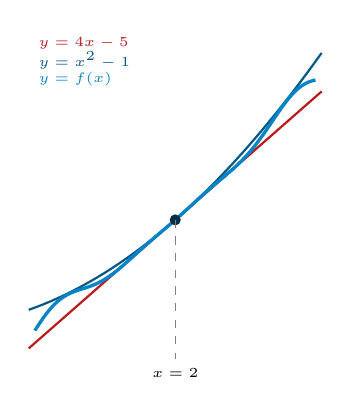
\begin{tikzpicture}[x=1.55cm,y=0.34cm]
\draw[brick,thick,domain=0.8:3.2] plot(\x,{4*\x-5});
\draw[mainc,thick,domain=0.8:3.2,samples=40] plot(\x,{\x*\x-1});
\draw[accc,very thick,domain=0.85:3.15,samples=120] plot(\x,{4*\x-5+(\x-2)*(\x-2)*(0.5+0.45*sin(deg(7*\x)))});
\fill[deepc] (2,3) circle (2pt);
\draw[dashed,gray] (2,3)--(2,-2.2);
\node[font=\tiny,below] at (2,-2.2) {$x=2$};
\node[anchor=north west,font=\tiny,align=left] at (0.8,10.2) {\textcolor{brick}{$y=4x-5$}\\ \textcolor{mainc}{$y=x^2-1$}\\ \textcolor{accc}{$y=f(x)$}};
\end{tikzpicture}}}{\pil{$3$}{$4$}{$5$}{$6$}{tidak dapat ditentukan}}
\soal{Fungsi $f(x)=\begin{cases}\dfrac{x^2-9}{x-3}, & x<3\\[2mm] a, & x=3\\[1mm] \dfrac{b\left(\sqrt{x+6}-3\right)}{x-3}, & x>3\end{cases}$ kontinu di $x=3$. Nilai $a+b$ adalah \dots.}{\pil{$12$}{$42$}{$48$}{$54$}{$72$}}

\tingkat{Tingkat Sulit}{soal 12 sampai 18}
\soal{Diketahui $\dis\lim_{x\to\infty}\left(\sqrt{ax^2+bx+1}-(2x-1)\right)=3$. Nilai $a+b$ adalah \dots.}{\pil{$4$}{$8$}{$10$}{$12$}{$16$}}
\soal{Nilai $\dis\lim_{x\to0}\dfrac{1-\cos x\cos2x}{x^2}$ adalah \dots.}{\pil{$\frac32$}{$2$}{$\frac52$}{$3$}{$\frac72$}}
\soal{\gbr{Grafik fungsi $f$ ditunjukkan pada gambar. Misalkan $g(x)=2-(x-1)^2$ dan $h(x)=2+(x-1)^2$. Nilai $\dis\lim_{x\to1}\Big[f\big(g(x)\big)-f\big(h(x)\big)\Big]$ adalah \dots.}{%
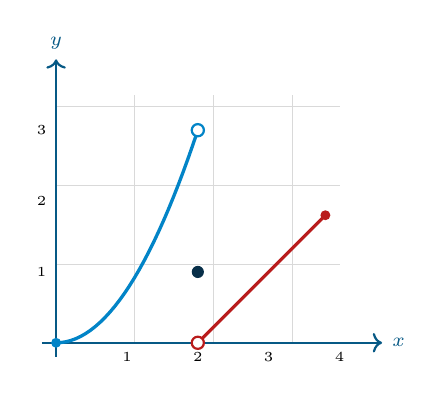
\begin{tikzpicture}[x=0.9cm,y=0.9cm]
\draw[gray!30] (0,0) grid (4,3.5);
\draw[->,thick,mainc] (-0.2,0)--(4.6,0) node[right,font=\scriptsize]{$x$};
\draw[->,thick,mainc] (0,-0.2)--(0,4) node[above,font=\scriptsize]{$y$};
\draw[accc,very thick,domain=0:2,samples=30] plot(\x,{0.75*\x*\x});
\draw[brick,very thick] (2,0)--(3.8,1.8);
\fill[accc] (0,0) circle (1.8pt);
\fill[brick] (3.8,1.8) circle (1.8pt);
\draw[fill=white,draw=accc,thick] (2,3) circle (2.2pt);
\draw[fill=white,draw=brick,thick] (2,0) circle (2.2pt);
\fill[deepc] (2,1) circle (2.2pt);
\foreach \i in {1,2,3}{\node[font=\tiny,left] at (0,\i){$\i$};}
\foreach \i in {1,2,3,4}{\node[font=\tiny,below] at (\i,0){$\i$};}
\end{tikzpicture}}}{\pil{$2$}{$3$}{$4$}{$6$}{tidak ada}}
\soal{Fungsi $f$ terdiferensialkan di $x=3$ dengan $f(3)=2$ dan $f'(3)=5$. Nilai $\dis\lim_{h\to0}\dfrac{\big[f(3+2h)\big]^2-\big[f(3-h)\big]^2}{h}$ adalah \dots.}{\pil{$15$}{$20$}{$30$}{$40$}{$60$}}
\soal{Nilai $\dis\lim_{x\to\pi/3}\dfrac{1-2\cos x}{\pi-3x}$ adalah \dots.}{\pil{$-\frac{\sqrt3}{3}$}{$-\sqrt3$}{$-\frac13$}{$\frac{\sqrt3}{3}$}{$\sqrt3$}}
\soal{\gbr{Perhatikan grafik fungsi $f(x)=x\left\lfloor\dfrac1x\right\rfloor$ untuk $0<x\le1$ pada gambar. Nilai $\dis\lim_{x\to0^+}f(x)$ adalah \dots.}{%
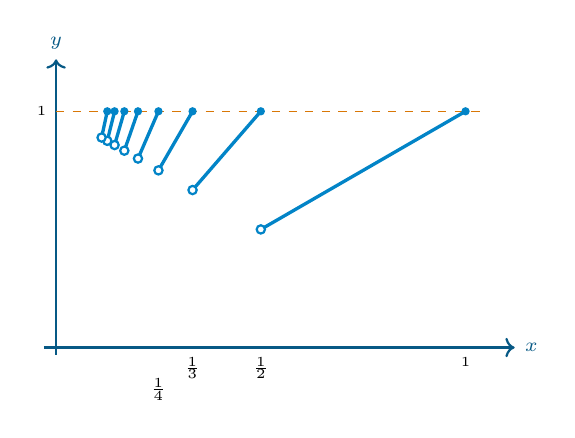
\begin{tikzpicture}[x=5.2cm,y=3cm]
\draw[->,thick,mainc] (-0.03,0)--(1.12,0) node[right,font=\scriptsize]{$x$};
\draw[->,thick,mainc] (0,-0.03)--(0,1.22) node[above,font=\scriptsize]{$y$};
\draw[warmc,dashed] (0,1)--(1.05,1);
\node[font=\tiny,left] at (0,1) {$1$};
\foreach \k in {1,...,8}{
 \draw[accc,very thick] ({1/(\k+1)},{\k/(\k+1)})--({1/\k},1);
 \draw[fill=white,draw=accc,thick] ({1/(\k+1)},{\k/(\k+1)}) circle (1.5pt);
 \fill[accc] ({1/\k},1) circle (1.5pt);}
\node[font=\tiny,below] at (1,0) {$1$};
\node[font=\tiny,below] at (0.5,0) {$\frac12$};
\node[font=\tiny,below] at (0.333,0) {$\frac13$};
\node[font=\tiny,below] at (0.25,-0.09) {$\frac14$};
\end{tikzpicture}}}{\pil{$0$}{$\frac12$}{$1$}{$2$}{tidak ada}}
\soal{Nilai $\dis\lim_{x\to-\infty}\left(\sqrt{x^2+4x}+x\right)$ adalah \dots.}{\pil{$-2$}{$-1$}{$0$}{$1$}{$2$}}

\tingkat{Tingkat HOTS}{soal 19 dan 20, penalaran tingkat tinggi}
\soal{Diketahui $\dis\lim_{x\to2}\dfrac{x^2+ax+b}{x^2-4}$ ada sebagai bilangan real. Berapakah nilai limit tersebut?
\begin{enumerate}[label=(\arabic*),leftmargin=1.8em,itemsep=0pt,topsep=2pt]
\item $a=-6$.
\item $b=8$.
\end{enumerate}}{\begin{tabularx}{\linewidth}{@{}lX@{}}
\textbf{A.} & Pernyataan (1) SAJA cukup untuk menjawab pertanyaan, tetapi pernyataan (2) SAJA tidak cukup.\\
\textbf{B.} & Pernyataan (2) SAJA cukup untuk menjawab pertanyaan, tetapi pernyataan (1) SAJA tidak cukup.\\
\textbf{C.} & DUA pernyataan BERSAMA-SAMA cukup untuk menjawab pertanyaan, tetapi SATU pernyataan SAJA tidak cukup.\\
\textbf{D.} & Pernyataan (1) SAJA cukup dan pernyataan (2) SAJA cukup untuk menjawab pertanyaan.\\
\textbf{E.} & Pernyataan (1) dan pernyataan (2) tidak cukup untuk menjawab pertanyaan.
\end{tabularx}}
\soal{\gbr{Pada lingkaran satuan berpusat di $O$, titik $A$ dan $B$ terletak pada lingkaran dengan $\angle AOB=\theta$ (radian), $0<\theta<\pi$. Titik $M$ adalah titik tengah busur kecil $AB$. Misalkan $S(\theta)$ luas segmen (daerah antara busur $AB$ dan tali busur $AB$) dan $T(\theta)$ luas segitiga $ABM$. Nilai $\dis\lim_{\theta\to0^+}\dfrac{S(\theta)}{T(\theta)}$ adalah \dots.\par\smallskip\footnotesize (Petunjuk: nyatakan $S$ dan $T$ dalam $\tfrac\theta2$.)}{%
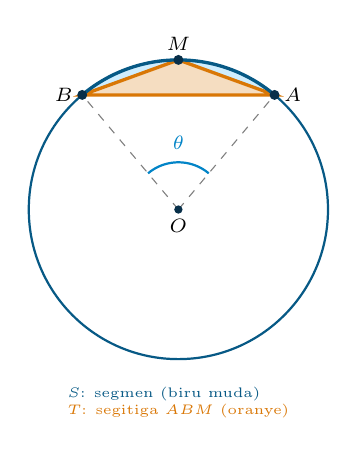
\begin{tikzpicture}
\def\r{1.9}
\coordinate (O) at (0,0);
\coordinate (A) at ({\r*cos(50)},{\r*sin(50)});
\coordinate (B) at ({\r*cos(130)},{\r*sin(130)});
\coordinate (M) at (0,\r);
\draw[mainc,thick] (O) circle (\r);
\fill[skyl,opacity=0.7] (A) arc (50:130:\r) -- cycle;
\draw[warmc,very thick,fill=warmc!25] (A)--(B)--(M)--cycle;
\draw[mainc,very thick] (A) arc (50:130:\r);
\draw[gray,dashed] (O)--(A) (O)--(B);
\draw[accc,thick] (50:0.6) arc (50:130:0.6);
\node[font=\scriptsize,accc] at (90:0.85) {$\theta$};
\fill[deepc] (O) circle (1.5pt) (A) circle (1.8pt) (B) circle (1.8pt) (M) circle (1.8pt);
\node[font=\scriptsize,right] at (A) {$A$};
\node[font=\scriptsize,left] at (B) {$B$};
\node[font=\scriptsize,above] at (M) {$M$};
\node[font=\scriptsize,below] at (O) {$O$};
\node[font=\tiny,align=left] at (0,-2.45) {\textcolor{mainc}{$S$: segmen (biru muda)}\\ \textcolor{warmc}{$T$: segitiga $ABM$ (oranye)}};
\end{tikzpicture}}}{\pil{$\frac12$}{$\frac23$}{$1$}{$\frac32$}{$\frac43$}}

% =====================================================================
\Needspace{14\baselineskip}
\bagian{B. Isian Singkat}{5 soal $\times$ 4 poin = 20 poin. Tuliskan hanya jawaban akhir.}

\tingkat{Tingkat Sedang}{soal 1 dan 2}
\soal{Nilai $\dis\lim_{x\to0}\dfrac{3x+\sin2x}{5x-\tan x}$ adalah \dots.}{\jwb}
\soal{Nilai $\dis\lim_{x\to\infty}\left(\sqrt{4x^2-3x+1}-(2x+1)\right)$ adalah \dots.}{\jwb}

\tingkat{Tingkat Sulit}{soal 3 sampai 5}
\soal{Nilai $\dis\lim_{x\to0}\dfrac{\sqrt{1+6x}\,\sqrt[3]{1+9x}\,\sqrt[4]{1+8x}-1}{x}$ adalah \dots.}{\jwb}
\soal{Nilai $\dis\lim_{x\to\infty}\left(\dfrac{x^2+3x}{x^2-x}\right)^{x}$ adalah \dots.}{\jwb}
\soal{Nilai $\dis\lim_{x\to\infty}x\Big(\sqrt{x^2+2x}-(x+1)\Big)$ adalah \dots.}{\jwb}

% =====================================================================
\Needspace{16\baselineskip}
\bagian{C. Uraian (Essay)}{5 soal $\times$ 8 poin = 40 poin. Tuliskan langkah penyelesaian dengan lengkap.}

\tingkat{Tingkat Sedang}{soal 1 dan 2}
\soal{\gbr{Fungsi $f$ didefinisikan oleh
\[f(x)=\begin{cases}\dfrac{x^2-x-2}{x-2}, & x<2\\[2mm] k, & x=2\\[1mm] \dfrac{24\left(\sqrt{x+7}-3\right)}{x-2}, & x>2\end{cases}\]
dengan $k$ konstanta (lihat gambar).\par\smallskip
(a) Tentukan $\dis\lim_{x\to2^-}f(x)$.\par
(b) Tentukan $\dis\lim_{x\to2^+}f(x)$.\par
(c) Adakah nilai $k$ sehingga $f$ kontinu di $x=2$? Jelaskan, dan sebutkan jenis ketakkontinuannya.\par
(d) Bilangan $24$ pada cabang kanan diganti dengan $m$. Tentukan $m$ dan $k$ agar $f$ kontinu di $x=2$, lalu hitung $\dis\lim_{x\to\infty}f(x)$ untuk nilai $m$ tersebut.}{%
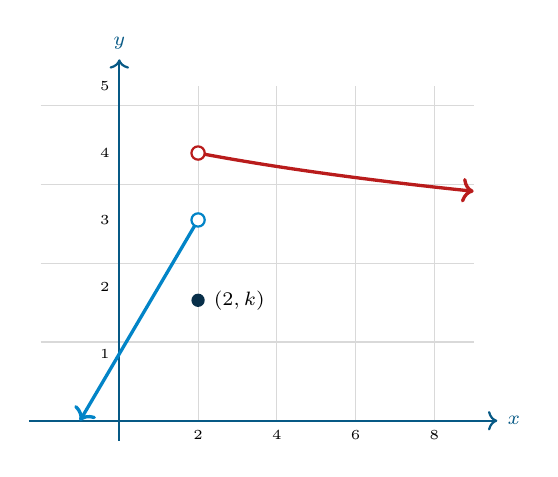
\begin{tikzpicture}[x=0.5cm,y=0.85cm]
\draw[gray!30] (-2,0) grid (9,5);
\draw[->,thick,mainc] (-2.3,0)--(9.6,0) node[right,font=\scriptsize]{$x$};
\draw[->,thick,mainc] (0,-0.3)--(0,5.4) node[above,font=\scriptsize]{$y$};
\draw[accc,very thick,<-] (-1,0)--(2,3);
\draw[brick,very thick,->,domain=2:9,samples=30] plot(\x,{24/(sqrt(\x+7)+3)});
\draw[fill=white,draw=accc,thick] (2,3) circle (2.4pt);
\draw[fill=white,draw=brick,thick] (2,4) circle (2.4pt);
\fill[deepc] (2,1.8) circle (2.4pt);
\node[font=\scriptsize,right] at (2.15,1.8) {$(2,k)$};
\foreach \i in {1,2,3,4,5}{\node[font=\tiny,left] at (0,\i){$\i$};}
\foreach \i in {2,4,6,8}{\node[font=\tiny,below] at (\i,0){$\i$};}
\end{tikzpicture}}}{\poin{8}}
\soal{\gbr{Laju reaksi suatu enzim $v$ (mikromol/menit) bergantung pada konsentrasi zat $s$ (mM) menurut
\[v(s)=\dfrac{12s}{3+s},\qquad s\ge0,\]
dengan grafik seperti pada gambar.\par\smallskip
(a) Tentukan $\dis\lim_{s\to\infty}v(s)$ dan jelaskan artinya bagi laju reaksi.\par
(b) Tentukan konsentrasi $s$ agar laju reaksi mencapai setengah dari nilai limit pada (a).\par
(c) Hitung $\dis\lim_{s\to0^+}\dfrac{v(s)}{s}$ dan jelaskan arti geometrisnya pada grafik.\par
(d) Tentukan konsentrasi terkecil agar laju reaksi mencapai $95\%$ dari nilai limit pada (a).}{%
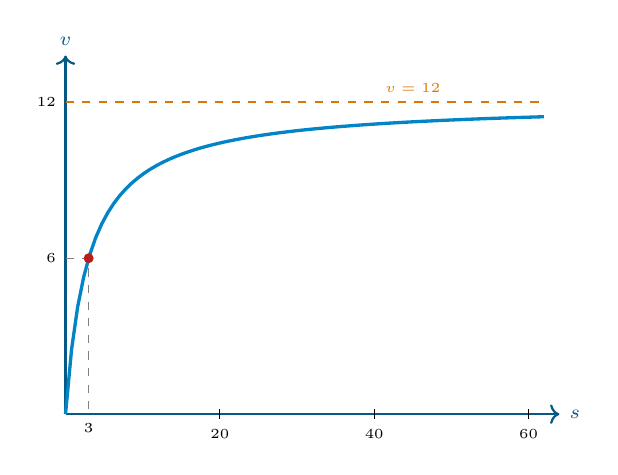
\begin{tikzpicture}[x=0.098cm,y=0.33cm]
\draw[->,thick,mainc] (0,0)--(64,0) node[right,font=\scriptsize]{$s$};
\draw[->,thick,mainc] (0,0)--(0,13.8) node[above,font=\scriptsize]{$v$};
\draw[dashed,warmc,thick] (0,12)--(62,12);
\node[font=\tiny,warmc,above] at (45,12) {$v=12$};
\draw[accc,very thick,domain=0:62,samples=80] plot(\x,{12*\x/(3+\x)});
\draw[dashed,gray] (0,6)--(3,6)--(3,0);
\fill[brick] (3,6) circle (1.8pt);
\node[font=\tiny,left] at (0,6) {$6$};
\node[font=\tiny,left] at (0,12) {$12$};
\node[font=\tiny,below] at (3,0) {$3$};
\foreach \i in {20,40,60}{\draw (\i,0.2)--(\i,-0.2) node[below,font=\tiny]{$\i$};}
\end{tikzpicture}}}{\poin{8}}

\Needspace{22\baselineskip}
\tingkat{Tingkat Sulit}{soal 3 dan 4}
\soal{\gbr{Pada lingkaran satuan berpusat di $O$ terdapat titik $A(1,0)$ dan titik $B$ dengan $\angle AOB=\theta$, $0<\theta<\frac\pi2$. Garis $OB$ memotong garis singgung lingkaran di $A$ pada titik $T$, sehingga $AT=\tan\theta$ (lihat gambar).\par\smallskip
(a) Nyatakan luas segitiga $OAB$, juring $OAB$, dan segitiga $OAT$ dalam $\theta$, lalu tuliskan hubungan urutan ketiganya.\par
(b) Dari (a), turunkan ketidaksamaan $\cos\theta<\dfrac{\sin\theta}{\theta}<1$.\par
(c) Gunakan Teorema Apit untuk menyimpulkan $\dis\lim_{\theta\to0^+}\dfrac{\sin\theta}{\theta}=1$, lalu jelaskan mengapa limit dua arahnya juga $1$.\par
(d) Dengan hasil (c), hitung $\dis\lim_{\theta\to0}\dfrac{1-\cos\theta}{\theta^2}$ tanpa memakai aturan L'H\^opital.}{%
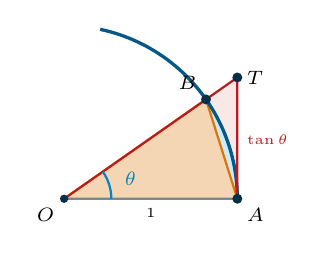
\begin{tikzpicture}
\def\r{2.2}\def\a{35}
\coordinate (O) at (0,0);
\coordinate (A) at (\r,0);
\coordinate (B) at ({\r*cos(\a)},{\r*sin(\a)});
\coordinate (T) at (\r,{\r*tan(\a)});
\fill[brick!10] (O)--(A)--(T)--cycle;
\fill[skyl!80] (O)--(A) arc (0:\a:\r)--cycle;
\draw[warmc,thick,fill=warmc!30] (O)--(A)--(B)--cycle;
\draw[mainc,very thick] (A) arc (0:78:\r);
\draw[brick,thick] (O)--(T)--(A);
\draw[gray] (O)--(A);
\draw[accc,thick] (0.6,0) arc (0:\a:0.6);
\node[font=\scriptsize,accc] at (17:0.88) {$\theta$};
\fill[deepc] (O) circle (1.5pt) (A) circle (1.8pt) (B) circle (1.8pt) (T) circle (1.8pt);
\node[font=\scriptsize,below left] at (O) {$O$};
\node[font=\scriptsize,below right] at (A) {$A$};
\node[font=\scriptsize,above left] at (B) {$B$};
\node[font=\scriptsize,right] at (T) {$T$};
\node[font=\tiny,below] at (1.1,0) {$1$};
\node[font=\tiny,right,brick] at (\r,0.75) {$\tan\theta$};
\end{tikzpicture}}}{\poin{8}}
\soal{\gbr{Misalkan
\[f(x)=\dfrac{x^3+ax^2+bx-4}{(x-1)^2}\]
dan diketahui $\dis\lim_{x\to1}f(x)=L$ ada sebagai bilangan real (lihat gambar untuk gambaran grafiknya).\par\smallskip
(a) Jelaskan mengapa pembilang habis dibagi $(x-1)$, dan tentukan hubungan antara $a$ dan $b$.\par
(b) Setelah dibagi $(x-1)$, jelaskan syarat tambahan agar limit tetap berhingga, lalu tentukan $a$ dan $b$.\par
(c) Tentukan $L$ dan jelaskan bentuk grafik $y=f(x)$.\par
(d) Jika penyebut diganti menjadi $(x-1)^3$ dengan $a$ dan $b$ yang sama, selidiki limit kiri dan limit kanan di $x=1$.}{%
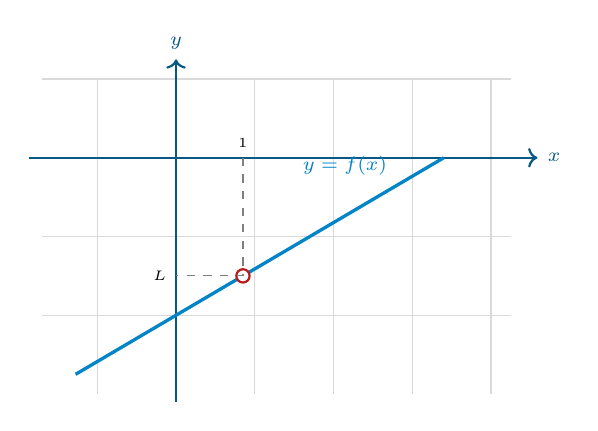
\begin{tikzpicture}[x=0.85cm,y=0.5cm]
\draw[gray!30] (-2,-6) grid (5,2);
\draw[->,thick,mainc] (-2.2,0)--(5.4,0) node[right,font=\scriptsize]{$x$};
\draw[->,thick,mainc] (0,-6.2)--(0,2.5) node[above,font=\scriptsize]{$y$};
\draw[accc,very thick] (-1.5,-5.5)--(4,0);
\draw[fill=white,draw=brick,thick] (1,-3) circle (2.4pt);
\draw[dashed,gray] (1,0)--(1,-3)--(0,-3);
\node[font=\tiny,left] at (0,-3) {$L$};
\node[font=\tiny,above] at (1,0) {$1$};
\node[font=\scriptsize,accc,above left] at (3.3,-0.7) {$y=f(x)$};
\end{tikzpicture}}}{\poin{8}}

\Needspace{26\baselineskip}
\tingkat{Tingkat HOTS}{soal 5}
\soal{\gbr{Fungsi $f:\mathbb R\to\mathbb R$ didefinisikan oleh
\[f(x)=\begin{cases}x, & x\text{ rasional}\\ x^2, & x\text{ irasional}\end{cases}\]
Grafiknya terdiri atas dua kurva yang masing-masing hanya ``berisi'' titik-titik dengan absis rasional atau irasional (lihat gambar).\par\smallskip
(a) Buktikan $\dis\lim_{x\to0}f(x)=0$ dengan Teorema Apit. (Petunjuk: untuk $|x|<1$ berlaku $x^2\le|x|$.)\par
(b) Buktikan $\dis\lim_{x\to1}f(x)=1$. (Petunjuk: bandingkan $|f(x)-1|$ dengan $|x-1|$ untuk $x$ dekat $1$.)\par
(c) Tunjukkan bahwa untuk setiap $a\notin\{0,1\}$, $\dis\lim_{x\to a}f(x)$ tidak ada. (Gunakan dua barisan, satu rasional dan satu irasional, yang menuju $a$.) Di titik mana saja $f$ kontinu?\par
(d) Selidiki apakah $f'(0)$ ada.}{%
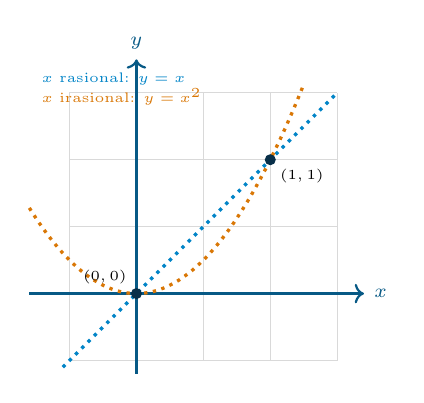
\begin{tikzpicture}[x=1.7cm,y=1.7cm]
\draw[gray!30] (-0.5,-0.5) grid[step=0.5] (1.5,1.5);
\draw[->,thick,mainc] (-0.8,0)--(1.7,0) node[right,font=\scriptsize]{$x$};
\draw[->,thick,mainc] (0,-0.6)--(0,1.75) node[above,font=\scriptsize]{$y$};
\draw[accc,dotted,very thick] (-0.55,-0.55)--(1.5,1.5);
\draw[warmc,dotted,very thick,domain=-0.8:1.25,samples=60] plot(\x,{\x*\x});
\fill[deepc] (0,0) circle (2pt) (1,1) circle (2pt);
\node[font=\tiny,above left] at (0,0) {$(0,0)$};
\node[font=\tiny,below right] at (1,1) {$(1,1)$};
\node[anchor=north west,font=\tiny,align=left] at (-0.78,1.72) {\textcolor{accc}{$x$ rasional: $y=x$}\\ \textcolor{warmc}{$x$ irasional: $y=x^2$}};
\end{tikzpicture}}}{\poin{8}}

% =====================================================================
\newpage
\bagian{Kunci Jawaban dan Pembahasan Singkat}{Untuk guru dan pembahasan mandiri}
\par\vspace{0.6em}{\bfseries\color{mainc}Kunci Pilihan Ganda}\par\vspace{0.3em}
\small
\begin{tabularx}{\linewidth}{@{}*{10}{>{\centering\arraybackslash}X}@{}}\hline \textbf{1} & \textbf{2} & \textbf{3} & \textbf{4} & \textbf{5} & \textbf{6} & \textbf{7} & \textbf{8} & \textbf{9} & \textbf{10}\\ \hline D & C & B & E & A & B & C & E & D & A\\ \hline\end{tabularx}\\[6pt]
\begin{tabularx}{\linewidth}{@{}*{10}{>{\centering\arraybackslash}X}@{}}\hline \textbf{11} & \textbf{12} & \textbf{13} & \textbf{14} & \textbf{15} & \textbf{16} & \textbf{17} & \textbf{18} & \textbf{19} & \textbf{20}\\ \hline B & D & C & B & E & A & C & A & D & E\\ \hline\end{tabularx}
\par\vspace{0.4em}{\bfseries\color{mainc}Kunci Isian Singkat:}\ \ 1) $\frac54$\quad 2) $-\frac74$\quad 3) $8$\quad 4) $e^4$\quad 5) $-\frac12$
\par\vspace{0.8em}{\bfseries\color{mainc}\normalsize Pembahasan Pilihan Ganda}\par\vspace{0.2em}
\small\begin{enumerate}[leftmargin=2em,itemsep=2pt,topsep=2pt]
\item[\textbf{1.}] \textbf{(D)} Dari grafik: mendekati $x=2$ dari kiri nilai fungsi menuju $3$, dari kanan menuju $1$, dan $f(2)=2$ (titik penuh). Karena limit kiri $\ne$ limit kanan, $\lim\limits_{x\to2}f(x)$ tidak ada sehingga A dan B salah, dan $f$ tidak kontinu (E salah). C salah karena $1\ne2$. D benar: $3-1=2$.
\item[\textbf{2.}] \textbf{(C)} Dengan sifat limit: $\dfrac{4\cdot(-2)+6}{4-(-2)}=\dfrac{-2}{6}=-\dfrac13$.
\item[\textbf{3.}] \textbf{(B)} $\dfrac{(x+2)(x+3)}{(x-3)(x+2)}=\dfrac{x+3}{x-3}$ untuk $x\ne-2$, sehingga limitnya $\dfrac{1}{-5}=-\dfrac15$. (Jebakan: menjawab $0$ atau menyerah karena substitusi langsung membentuk $\frac00$.)
\item[\textbf{4.}] \textbf{(E)} Pembilang $2x^2+5x-3$ dan penyebut $3x^2-5x-2$ berderajat sama, sehingga limitnya perbandingan koefisien pangkat tertinggi: $\frac23$.
\item[\textbf{5.}] \textbf{(A)} (i) $\frac{\tan4x}{\sin2x}\to\frac42=2$, \textbf{B}. (ii) Karena $-1\le\sin x\le1$, maka $\left|\frac{\sin x}{x}\right|\le\frac1{|x|}\to0$ (Teorema Apit); limitnya $0$, bukan $1$, jadi \textbf{S}. (iii) Bagi dengan $x^2$: $\frac{2+1/x^2}{1-3/x^2}\to2$, \textbf{B}. Urutan: B, S, B.
\item[\textbf{6.}] \textbf{(B)} Kalikan sekawan pada masing-masing: $\sqrt{x+3}-2=\frac{x-1}{\sqrt{x+3}+2}$ dan $\sqrt{x+8}-3=\frac{x-1}{\sqrt{x+8}+3}$. Hasil bagi menjadi $\frac{\sqrt{x+8}+3}{\sqrt{x+3}+2}\to\frac{3+3}{2+2}=\frac32$. (Jebakan: terbalik menjadi $\frac23$.)
\item[\textbf{7.}] \textbf{(C)} Pakai $\lim\limits_{x\to0}\frac{1-\cos ax}{x^2}=\frac{a^2}2$. Tulis $\cos2x-\cos6x=(1-\cos6x)-(1-\cos2x)$, sehingga limitnya $\frac{36}2-\frac42=18-2=16$. Cek lewat $\cos2x-\cos6x=2\sin4x\sin2x$: $2\cdot4\cdot2=16$.
\item[\textbf{8.}] \textbf{(E)} $\frac{x+3}{x-1}=1+\frac4{x-1}$. Bentuk $\left(1+\frac4{x-1}\right)^{2x}=\left[\left(1+\frac4{x-1}\right)^{\frac{x-1}4}\right]^{\frac{8x}{x-1}}\to e^{8}$. (Jebakan: lupa pangkat $2$ sehingga $e^4$.)
\item[\textbf{9.}] \textbf{(D)} $PA-PB=\sqrt{(x+4)^2+4}-\sqrt{(x-2)^2+9}=\sqrt{x^2+8x+20}-\sqrt{x^2-4x+13}$. Dengan rumus selisih akar: $\frac{8-(-4)}{2\sqrt1}=6$. Secara geometris, untuk $x$ sangat besar $PA-PB$ mendekati selisih posisi mendatar kedua menara, yaitu $2-(-4)=6$; selisih tinggi ($3-2=1$) tidak berpengaruh.
\item[\textbf{10.}] \textbf{(A)} Saat $x\to2$: $4x-5\to3$ dan $x^2-1\to3$. Teorema Apit memberi $\lim\limits_{x\to2}f(x)=3$. (Garis $y=4x-5$ menyinggung parabola di $(2,3)$, karena $x^2-1-(4x-5)=(x-2)^2\ge0$.)
\item[\textbf{11.}] \textbf{(B)} Limit kiri: $\frac{x^2-9}{x-3}=x+3\to6$, sehingga $a=6$. Limit kanan: $\frac{b(\sqrt{x+6}-3)}{x-3}=\frac{b}{\sqrt{x+6}+3}\to\frac b6$. Kontinu berarti $\frac b6=6$, jadi $b=36$ dan $a+b=42$. (Jebakan: lupa pembagi $6$ sehingga $a+b=12$.)
\item[\textbf{12.}] \textbf{(D)} Agar limit berhingga, koefisien $x^2$ di bawah akar harus $p^2=4$, jadi $a=4$ (jika $a\ne4$, hasil menuju $\pm\infty$). Lalu $\sqrt{4x^2+bx+1}-(2x-1)=\frac{(b+4)x}{\sqrt{4x^2+bx+1}+2x-1}\to\frac{b+4}4=3$, sehingga $b=8$. Jadi $a+b=12$.
\item[\textbf{13.}] \textbf{(C)} $1-\cos x\cos2x=(1-\cos x)+\cos x\,(1-\cos2x)$. Bagi dengan $x^2$: $\frac{1-\cos x}{x^2}\to\frac12$ dan $\cos x\cdot\frac{1-\cos2x}{x^2}\to1\cdot\frac42=2$. Jumlah $\frac52$. (Jebakan: mengganti $\cos x$ dengan $1$ lebih dulu menghasilkan $2$.)
\item[\textbf{14.}] \textbf{(B)} Untuk $x\ne1$, $g(x)=2-(x-1)^2<2$ dan $g(x)\to2$, jadi $g(x)\to2^-$ dan $f(g(x))\to\lim\limits_{t\to2^-}f(t)=3$. Sedangkan $h(x)=2+(x-1)^2>2$, jadi $h(x)\to2^+$ dan $f(h(x))\to\lim\limits_{t\to2^+}f(t)=0$. Selisihnya $3-0=3$. (Limit $f$ di $2$ tidak ada dan $f(2)=1$ tidak berperan.)
\item[\textbf{15.}] \textbf{(E)} Misalkan $F=f^2$. Maka $F'(3)=2f(3)f'(3)=20$. Pisahkan: $\frac{F(3+2h)-F(3-h)}{h}=2\cdot\frac{F(3+2h)-F(3)}{2h}+\frac{F(3-h)-F(3)}{-h}\to2F'(3)+F'(3)=3F'(3)=60$. (Jebakan: $40$ bila suku kedua terlupa, $30$ bila lupa faktor $2$ pada $F'$.)
\item[\textbf{16.}] \textbf{(A)} Misalkan $t=x-\frac\pi3\to0$. $1-2\cos\left(t+\frac\pi3\right)=1-\cos t+\sqrt3\sin t$ dan $\pi-3x=-3t$. Limitnya $\dfrac{\frac{1-\cos t}{t}+\sqrt3\frac{\sin t}{t}}{-3}=\dfrac{0+\sqrt3}{-3}=-\dfrac{\sqrt3}{3}$.
\item[\textbf{17.}] \textbf{(C)} Untuk $x>0$: $\frac1x-1<\left\lfloor\frac1x\right\rfloor\le\frac1x$. Kalikan dengan $x>0$: $1-x<x\left\lfloor\frac1x\right\rfloor\le1$. Saat $x\to0^+$ kedua batas menuju $1$, sehingga limitnya $1$ (Teorema Apit). Jebakan: menjawab $0$ karena ``$x\to0$'', atau ``tidak ada'' karena grafik bergerigi.
\item[\textbf{18.}] \textbf{(A)} Untuk $x<0$, $\sqrt{x^2}=|x|=-x$. Kalikan sekawan: $\sqrt{x^2+4x}+x=\frac{4x}{\sqrt{x^2+4x}-x}$. Bagi pembilang dan penyebut dengan $-x>0$: pembilang $\to-4$, penyebut $\sqrt{1+\frac4x}+1\to2$. Limit $=-2$. (Jebakan: memakai hasil untuk $x\to+\infty$ yang memberi $2$.)
\item[\textbf{19.}] \textbf{(D)} Karena penyebut $\to0$ dan limit berhingga, pembilang harus $\to0$ di $x=2$: $4+2a+b=0$. Pernyataan (1): $a=-6\Rightarrow b=8$, pembilang $x^2-6x+8=(x-2)(x-4)$ dan limit $=\lim\frac{x-4}{x+2}=-\frac12$; cukup. Pernyataan (2): $b=8\Rightarrow a=-6$, hasil sama; cukup. Jadi masing-masing cukup.
\item[\textbf{20.}] \textbf{(E)} Misalkan $u=\frac\theta2$. Luas segmen $S=\frac{\theta-\sin\theta}{2}=u-\sin u\cos u=\frac12(2u-\sin2u)$. Untuk segitiga $ABM$: alas $AB=2\sin u$ dan tinggi dari $M$ ke tali busur $=1-\cos u$, sehingga $T=\sin u\,(1-\cos u)$. Dengan $\lim\limits_{x\to0}\frac{x-\sin x}{x^3}=\frac16$ (L'H\^opital tiga kali): $S\approx\frac12\cdot\frac{(2u)^3}{6}=\frac{2u^3}{3}$, sedangkan $T\approx u\cdot\frac{u^2}{2}=\frac{u^3}{2}$. Rasio $=\frac{2/3}{1/2}=\frac43$ (hasil klasik Archimedes untuk segmen parabola).
\end{enumerate}
\par\Needspace{6\baselineskip}\vspace{0.6em}{\bfseries\color{mainc}\normalsize Pembahasan Isian Singkat}\par\vspace{0.2em}
\small\begin{enumerate}[leftmargin=2em,itemsep=2pt,topsep=2pt]
\item[\textbf{1.}] \textbf{Jawaban: $\frac54$.} Bagi pembilang dan penyebut dengan $x$: $\frac{3+\frac{\sin2x}{x}}{5-\frac{\tan x}{x}}\to\frac{3+2}{5-1}=\frac54$.
\item[\textbf{2.}] \textbf{Jawaban: $-\frac74$.} Kalikan sekawan: $\sqrt{4x^2-3x+1}-(2x+1)=\frac{(4x^2-3x+1)-(2x+1)^2}{\sqrt{4x^2-3x+1}+2x+1}=\frac{-7x}{\sqrt{4x^2-3x+1}+2x+1}\to\frac{-7}{2+2}=-\frac74$. (Rumus: $\frac{b-2pq}{2p}=\frac{-3-4}{4}$.)
\item[\textbf{3.}] \textbf{Jawaban: $8$.} Misalkan $F(x)$ adalah hasil kali ketiga akar, $F(0)=1$. Limit yang diminta adalah $\lim\frac{F(x)-F(0)}{x}=F'(0)$. Karena tiap faktor bernilai $1$ di $x=0$, aturan hasil kali memberi $F'(0)=\frac62+\frac93+\frac84=3+3+2=8$. (Setara dengan $(1+kx)^{1/n}\approx1+\frac knx$ untuk $x$ kecil.)
\item[\textbf{4.}] \textbf{Jawaban: $e^4$.} $\frac{x^2+3x}{x^2-x}=1+\frac{4x}{x^2-x}=1+\frac4{x-1}$. Maka $\left(1+\frac4{x-1}\right)^x=\left[\left(1+\frac4{x-1}\right)^{\frac{x-1}4}\right]^{\frac{4x}{x-1}}\to e^4$.
\item[\textbf{5.}] \textbf{Jawaban: $-\frac12$.} Bentuk $\sqrt{x^2+2x}-(x+1)\to0$, tetapi dikalikan $x\to\infty$. Kalikan sekawan: $\sqrt{x^2+2x}-(x+1)=\frac{x^2+2x-(x+1)^2}{\sqrt{x^2+2x}+x+1}=\frac{-1}{\sqrt{x^2+2x}+x+1}$. Maka $x\cdot\frac{-1}{\sqrt{x^2+2x}+x+1}\to\frac{-1}{1+1}=-\frac12$.
\end{enumerate}
\par\Needspace{8\baselineskip}\vspace{0.6em}{\bfseries\color{mainc}\normalsize Pembahasan dan Pedoman Penskoran Uraian}\par\vspace{0.2em}
\small\begin{enumerate}[leftmargin=2em,itemsep=3pt,topsep=2pt]
\item[\textbf{1.}] (a) Untuk $x<2$: $\frac{x^2-x-2}{x-2}=\frac{(x-2)(x+1)}{x-2}=x+1\to3$. (b) $\sqrt{x+7}-3=\frac{x-2}{\sqrt{x+7}+3}$, sehingga $f(x)=\frac{24}{\sqrt{x+7}+3}\to\frac{24}{6}=4$. (c) Limit kiri $3\ne$ limit kanan $4$, jadi $\lim\limits_{x\to2}f(x)$ tidak ada; tidak ada nilai $k$ yang membuat $f$ kontinu di $2$. Ketakkontinuannya berjenis \emph{loncat} (selisih $1$), bukan ketakkontinuan yang dapat dihapus. (d) Kontinu menuntut $\frac m6=3$, sehingga $m=18$ dan $k=3$. Untuk $x>2$, $f(x)=\frac{18}{\sqrt{x+7}+3}$, penyebut $\to\infty$, jadi $\lim\limits_{x\to\infty}f(x)=0$ (garis $y=0$ asimtot mendatar di sisi kanan). \\ \textit{Penskoran: tiap bagian 2 poin.}
\item[\textbf{2.}] (a) $v(s)=\frac{12}{\frac3s+1}\to12$: laju reaksi tidak pernah melampaui $12$ dan mendekati laju maksimum (jenuh) $12$ mikromol/menit untuk konsentrasi yang sangat besar. (b) $\frac{12s}{3+s}=6\Rightarrow12s=18+6s\Rightarrow s=3$ mM. (c) $\frac{v(s)}{s}=\frac{12}{3+s}\to4$. Karena $v(0)=0$, nilai ini adalah kemiringan garis singgung grafik di titik asal, yaitu laju awal per satuan konsentrasi. (d) $\frac{12s}{3+s}\ge0{,}95\cdot12=11{,}4\Rightarrow12s\ge34{,}2+11{,}4s\Rightarrow0{,}6s\ge34{,}2\Rightarrow s\ge57$ mM. \\ \textit{Penskoran: tiap bagian 2 poin.}
\item[\textbf{3.}] (a) Luas segitiga $OAB=\frac12\cdot1\cdot1\cdot\sin\theta=\frac12\sin\theta$; juring $OAB=\frac12\cdot1^2\cdot\theta=\frac\theta2$; segitiga $OAT=\frac12\cdot OA\cdot AT=\frac12\tan\theta$. Segitiga $OAB$ termuat dalam juring dan juring termuat dalam segitiga $OAT$, sehingga $\frac12\sin\theta<\frac\theta2<\frac12\tan\theta$. (b) Kalikan $2$ dan bagi $\sin\theta>0$: $1<\frac\theta{\sin\theta}<\frac1{\cos\theta}$. Ambil kebalikan: $\cos\theta<\frac{\sin\theta}\theta<1$. (c) Saat $\theta\to0^+$, $\cos\theta\to1$ dan batas atas $1$, sehingga $\frac{\sin\theta}\theta\to1$. Fungsi $\frac{\sin\theta}{\theta}$ genap ($\frac{\sin(-\theta)}{-\theta}=\frac{\sin\theta}{\theta}$), jadi limit kirinya juga $1$ dan limit dua arahnya $1$. (d) $1-\cos\theta=2\sin^2\frac\theta2$, sehingga $\frac{1-\cos\theta}{\theta^2}=\frac12\left(\frac{\sin(\theta/2)}{\theta/2}\right)^2\to\frac12\cdot1^2=\frac12$. \\ \textit{Penskoran: tiap bagian 2 poin.}
\item[\textbf{4.}] (a) Penyebut $(x-1)^2\to0$. Agar hasil bagi berhingga, pembilang $N(x)=x^3+ax^2+bx-4$ harus $\to0$, yaitu $N(1)=a+b-3=0$, jadi $a+b=3$ dan $(x-1)$ adalah faktor $N$. (b) Pembagian $N$ oleh $(x-1)$ memberi $N(x)=(x-1)\left(x^2+(a+1)x+4\right)$ (karena $a+b+1=4$). Maka $f(x)=\frac{x^2+(a+1)x+4}{x-1}$ dan penyebut masih $\to0$, sehingga haruslah $x^2+(a+1)x+4\to0$ di $x=1$: $1+a+1+4=0\Rightarrow a=-6$, dan $b=9$. (c) $N(x)=x^3-6x^2+9x-4=(x-1)^2(x-4)$, sehingga $f(x)=x-4$ untuk $x\ne1$ dan $L=-3$. Grafiknya garis $y=x-4$ dengan lubang di titik $(1,-3)$. (d) $\frac{(x-1)^2(x-4)}{(x-1)^3}=\frac{x-4}{x-1}$. Saat $x\to1^+$: pembilang $\to-3$, penyebut $\to0^+$, hasilnya $-\infty$. Saat $x\to1^-$: penyebut $\to0^-$, hasilnya $+\infty$. Limit kiri dan kanan berbeda (tidak berhingga), sehingga limitnya tidak ada; $x=1$ menjadi asimtot tegak. \\ \textit{Penskoran: (a) 2 poin; (b) 3 poin; (c) 1 poin; (d) 2 poin.}
\item[\textbf{5.}] (a) Untuk $|x|<1$: jika $x$ rasional, $f(x)=x\in[-|x|,|x|]$; jika irasional, $f(x)=x^2\le|x|$ dan $x^2\ge0\ge-|x|$. Jadi $-|x|\le f(x)\le|x|$. Karena $\pm|x|\to0$, maka $\lim\limits_{x\to0}f(x)=0$. (b) Untuk $|x-1|<1$ (jadi $0<x<2$ dan $|x+1|<3$): jika $x$ rasional, $|f(x)-1|=|x-1|$; jika irasional, $|f(x)-1|=|x^2-1|=|x-1||x+1|<3|x-1|$. Jadi $1-3|x-1|\le f(x)\le1+3|x-1|$ dan limitnya $1$. (c) Ambil barisan rasional $r_n\to a$ dan barisan irasional $s_n\to a$ (selalu ada karena bilangan rasional dan irasional rapat). Maka $f(r_n)=r_n\to a$, sedangkan $f(s_n)=s_n^2\to a^2$. Karena $a\ne a^2$ untuk $a\notin\{0,1\}$, kedua barisan memberi limit berbeda sehingga $\lim\limits_{x\to a}f(x)$ tidak ada. Limit hanya ada di $a=0$ dan $a=1$, dan di sana nilainya sama dengan $f(0)=0$ dan $f(1)=1$; jadi $f$ kontinu tepat di $x=0$ dan $x=1$. (d) $\frac{f(x)-f(0)}{x}=\frac{f(x)}{x}$ bernilai $1$ untuk $x$ rasional dan $x$ untuk $x$ irasional. Untuk $x\to0$, nilai pertama tetap $1$ sedangkan nilai kedua $\to0$. Limitnya tidak ada, jadi $f'(0)$ tidak ada walaupun $f$ kontinu di $0$. \\ \textit{Penskoran: tiap bagian 2 poin.}
\end{enumerate}
\end{document}
